\section{Introduction}
The calculation of the optical response of diffraction gratings has been an active pursuit of electromagnetic research for over a century. In 1907, Lord Rayleigh proposed a treatment for the reflected light from periodic surfaces by considering them a perturbation of the case of a flat surface \cite{Rayleigh1907a}. This theory calculated that there must be a sharp discontinuity in the reflectivity from the grating when a diffracted order of light emerges from, or disappears beneath, the grating surface. This discontinuity, first observed experimentally as a dark band by Wood \cite{Light}, corresponds to the instances at which power must be redistributed to the propagating orders of light as a diffracted order either starts, or ceases, to propagate at the grating surface. However, Rayleigh's theory was inadequate for all but the shallowest gratings,  as it lacked a full consideration for the fields that could occur in the grating grooves. Furthermore, Rayleigh's treatment left the bright band observed by Wood, characteristic of a SPP excitation, unexplained.

Since 1907, many methods by which to model the optical response of gratings have been developed and have been verified experimentally. Methods such as Finite Difference Time domain methods and Fourier modal-matching methods have all been tested. A review of the these, and other, numerical methods of grating analysis can be found in reference \cite{Bao}.

The purpose of this chapter is to provide a background to the methods used in this thesis, namely the Finite Element Method (FEM) method and the coordinate transformation method of Chandezon et al. \cite{Chandezon1980}.

\section{The Differential Method of Chandezon et al.}
The method of Chandezon et al. \cite{Chandezon1980,Chandezon1982} solves Maxwell's equations by utilising a coordinate transformation which maps the grating interfaces on to flat, parallel, planes. This avoids the Rayleigh theory's failure to account fully for field inside the grooves, as the grating is effectively flattened by the coordinate transformation and the boundary conditions are then matched across this flat interface. For a monograting the transformed coordinates are,
\begin{align}
u&=x\label{eq:chandezon-orginalx}\\
w&=y\label{eq:chandezon-orginaly}\\
v&=z-S(x)\label{eq:chandezon-orginalz}
\end{align}
Where $S(x)$ is the interface profile of the grating. The ease of matching the boundary conditions in this modified frame is achieved at a cost of the need for more complex expressions for Maxwell's equations in a non-orthogonal coordinate system of $(u,v,w)$. In this method,  the derivation of the incident and  scattered fields from Maxwell's equations are expressed as an infinite series of plane waves, a Fourier expansion. 

In order to solve this problem numerically, the infinite Fourier series must be truncated, placing a limit on the number of scattered field components in the model. The order of truncation is chosen from a compromise between obtaining suitable convergence of the solution and minimising computation time. In this thesis, we primarily use Chandezon method modelling to provide illustrative examples of reflectivity by which we may explain certain observed optical features. For this purpose, we find that limiting the number of scattered fields in the system to 6 is sufficient.

The one-dimensional case was presented by Chandezon in 1980 \cite{Chandezon1980}. Since then, it has been extended to multi-layered gratings \cite{Cotter1995,Preist1995} and to bigratings \cite{Harris1996}. The method used in the thesis is the multi-layer bigrating method reported by Harris et al.\cite{Harris1996}. This allows for two crossed gratings of different pitches to be considered, and the coordinate transformation is altered from the equations \ref{eq:chandezon-orginalx}, \ref{eq:chandezon-orginaly} and \ref{eq:chandezon-orginalz} to,
\begin{align}
u&=x\\
w&=y'=x \cos{\alpha}+y \sin{\alpha}\\
v&=z-S(x,y')
\end{align}

Where $\alpha$ is the angle between the two crossed gratings.
This interface profile $S(x,y')$ is represented by a Fourier sum. Because the technique is a differential method, sharp discontinuities in the surface profile gradient are difficult to model. The number of Fourier components required to correctly simulate a step-like grating profile can become prohibitively large, although extensions to the method have shown than the method can be applied well to trapezium shaped grooves \cite{Chandezon2001}. For a precise description of a lamellar grating as produced by our fabrication techniques a large number of Fourier harmonics are required to represent $S(x,y')$, which can make computation times prohibitively long. However for the grating periodicities used in this thesis only the dominant scattering associated with low order Fourier components need be considered to gain sufficient insight into the underlying physical processes.

The Chandezon method has been used successfully to probe the electromagnetic response of hexagonal bigratings \cite{Watts1996}, the effect of groove shape on reflectivity resonances due to SPP excitations \cite{Watts1998,Watts1999}, to examine asymmetric excitation of SPPs on blazed gratings \cite{Bai2009} and to determine the surface profile of gratings from experimentally acquired reflectivity measurements \cite{T.Hallam2000}. 


\section{The Finite Element Method}

The finite element method (FEM) \nomenclature{FEM}{The Finite Element Method for calculating the optical response of a system.} for predicting the electromagnetic response of systems is a numerical modelling process that subdivides a system into discrete elements, solving Maxwell's equations for each element and ensuring the solutions are consistent across each elementary boundary \cite{Press,Bao}. 
Broadly, the process iteratively applies three steps until a solution is found: 
\begin{enumerate}
\item{Determining the distribution and size of elements across the model. The continuous array of elements is referred to as the `mesh' of the model.}
\item{
Numerically solving Maxwell's equations for each element and for the mesh as a whole.}
\item{The evaluation of the quality of the solution, to see if the model converges to a consistent and physically accurate solution. If not, the process repeats from (1), further refining the mesh.}
\end{enumerate}

The software package used for FEM modelling in this thesis is the HFSS package from Ansys, Inc. \cite{Ansys2012}. The software includes a computer aided design component, which allows the building of three-dimensional models  to represent the sample under consideration. These 3D models may be assigned different optical parameters, such as frequency-dependent permittivities and permeabilities, and may be parametrised for automated parametric alterations. The software's default element shape is a tetrahedron, with many tetrahedra forming a conformal mesh in the problem domain. In the case of 3D models which contain curved surfaces, the software may also use curvilinear tetrahedral elements, greatly reducing the number of elements required to approximate a curved surface.

\subsection{Solving Maxwell's Equations in the Mesh}
The FEM package attempts to solve for the electric field \cite{Kopp2009}, $\mathbf{E}$, for each element using the wave equation,
\begin{equation}
	\mathbf{\nabla} \times \left( \frac{1}{\mu} \mathbf{\nabla} \times 	\mathbf{E} \right) -k_0^2 \varepsilon \mathbf{E} = 0
	\label{eq:hfss-efield}
\end{equation}
where $k_0$ is the free space wavenumber and $\varepsilon$ and $\mu$ are the relative permittivity and relative permeability, respectively. As a numerical simulation, the software attempts to minimise the left hand side of equation \ref{eq:hfss-efield} to be as close to zero as possible for each element, it will not in general, equal exactly zero. The magnetic field, $\mathbf{H}$ is then calculated using,
\begin{equation}
	\mathbf{H}=\frac{1}{\omega \mu} \mathbf{\nabla} \times \mathbf{E}
\end{equation}
where $\omega$ is the angular frequency of the wave. The values for $\mathbf{E}$ and $\mathbf{H}$ must be found for all the elements forming the conformal mesh in the problem space, and must be consistent across each tetrahedron boundary. This leads to thousands of simultaneous equations in the form of equation \ref{eq:hfss-efield} for each finite element in the model, which are combined into a matrix and solved for $\mathbf{E}$ numerically.

Once the fields have been determined, a generalised scattering matrix (S-Matrix) is derived for the system, from which initial and final optical properties such as reflectivity or transmission can be extracted. The software may also attempt to find the frequencies at which the poles of the S-Matrix occur, and so calculate the eigenmodes of the system and their associated fields.

\subsection{Adaptive Meshing}

The structure of the mesh used in the FEM model is critical to obtaining an accurate simulation. In general, a higher resolution of mesh is required in areas where the electric (and magnetic) field vary rapidly. To achieve a suitable mesh, the FEM package uses a process of adaptive meshing, refining the mesh in areas where the error in the electric field calculation are high.

In the process, the software generates an initial, geometrically conformal mesh, and solves equation \ref{eq:hfss-efield} for the electric field for each of the tetrahedra. Based on this initial solution, the area of the problem domain where the exact solution has a large amount of error is determined \cite{Kopp2009}. This is done by examining the residuals of equation \ref{eq:hfss-efield}, such that the approximate solution, $\mathbf{E}_{approx}$ gives,
\begin{equation}
	\mathbf{\nabla} \times \left( \frac{1}{\mu} \mathbf{\nabla} \times 	\mathbf{E}_{approx} \right) -k_0^2 \varepsilon \mathbf{E}_{approx} = residual
\end{equation}
for each tetrahedron. A set percentage of tetrahedra with the largest residuals are then refined by sub-dividing the element into even smaller tetrahedra. Another solution is then found with this new mesh, and the process  is repeated until the convergence criteria has been met, or the total number of adaptive passes, set by the user to prevent overly complex and memory intensive meshes, has been met.

It is important to note that the simple addition of elements to the problem is inefficient, and that the software's determination of the refinement areas by consideration of highest tetrahedral residuals is not foolproof. Occasionally, the software may attempt to refine the mesh in locations that are not critical, but do lie in the upper percentile of tetrahedral locations with high residuals. Users can make the simulation more efficient by defining the initial mesh conditions using mesh operations in the software. For example, someone setting up a simulation for plasmonic resonances in thin cavities may start the initial mesh with a greater density of elements in the grooves (where they expect rapidly varying fields) than the software alone might allocate.


\subsection{Solution Evaluation and Convergence}

The accuracy of the solution is determined by the model's `convergence'. Because of the direct relationship between the electric fields for a solution and the corresponding S-Matrix,  the convergence is measured by the change in the magnitude of two successive solutions and is called the $\Delta S$ value. It is a measure of the change in electric field distribution between solutions. When the $\Delta S$ values becomes less than a user-specified amount, the model is deemed to be `converged' and the final solution is obtained. An example of mesh refinement is shown in figure \ref{fig:hfssconvergence}. 
\begin{figure}[h]
	\begin{center}
		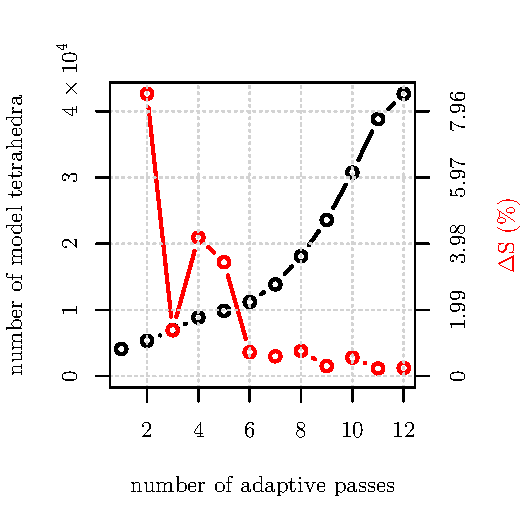
\includegraphics{figure-convergence.pdf}
		\caption[A graph showing the convergence of a typical FEM model as a function of adaptive passes.]{A graph showing the convergence of a typical FEM model as a function of adaptive passes. The black line shows the total number of elements introduced in the model, while the \color{red} red \color{black}line shows the $\Delta S$ parameter as a percentage.\label{fig:hfssconvergence}}
	\end{center}
\end{figure}
Here, we find that the refinement algorithm adds more elements to the mesh, to a total of over 40,000 in the final case, in order to reduce the $\Delta S$ value (red line) and achieve convergence. This particular example is the convergence for a zigzag grating model, the results of which are detailed in chapter \ref{c:zigzag}. For the results in this thesis, the maximum $\Delta S$ value used was 2\%.


\subsection{Model Boundary Conditions}
\begin{figure}[h]
\begin{center}
\input{figure-hfssboundary.eps_tex}
\end{center}
\caption[Schematic of the different boundaries used in the FEM model.]{Schematic of the different boundaries used in the FEM model. The unit cell shown is a zigzag grating (chapter \ref{c:zigzag}) in red. The boundaries are highlighted and named in each case. The Perfect E boundary has been extruded from the bottom of the model for clarity.}\label{fig:hfssunitcell}
\end{figure}
In the FEM package, the modelled system must be surrounded by appropriate boundary conditions so a solution can be determined. Diffraction gratings in this thesis are approximated to infinite periodic structures, as the propagation lengths of SPPs is far smaller than the sample size. Thus, a unit cell of the structure with appropriate boundary conditions is suitable for a full solution to the problem, an example being shown in figure \ref{fig:hfssunitcell}. This unit cell is surrounded by 4 types of boundary, labelled in the figure.
The first type is called a master-slave boundary. This boundary pair constrains  the electric and magnetic field so that fields at the master boundary must match exactly the field at the slave boundary. The periodic boundary conditions imposed by the master-slave pair ensure that the solution is exactly equivalent to an infinite array of unit cells. The slave boundary may also replicate the fields at the master with an additional relative phase delay. This phase delay is how the software calculates the fields for an angle of incidence other than normal with the phase delay calculated internally from the provided polar and azimuthal angles.
The next type of boundary is the `Perfect E' boundary. This boundary acts as a perfect lossless conductor. It is placed on the bottom of the metal film, and acts as an easy way to double the thickness of the metal film by reflecting perfectly any impinging radiation. Since the field penetration for visible radiation in to a metal such a silver is very small (on the order of 20 nm), a metal film thickness of 50 nm, used together with the Perfect E boundary, provides a suitable approximation to a semi-infinite metal substrate without the additional cost of increasing the number of tetrahedra.
The final boundary is a Floquet port. This acts as a radiation boundary that is open to free-space. The FEM package actually absorbs any radiation that hits this boundary, without reflection, mimicking the character of radiation escaping to free-space. This Floquet port also acts as an excitation source and a way by which certain orders of diffracted field are extracted, which is covered in the next subsection.

\subsection{Floquet Type Excitation}
When extracting the reflectivity of a diffracting sample from the S-Matrix, it becomes clear that simply examining the total field arriving above the sample does not correspond meaningfully to the types of experiments typically conducted in this thesis. This is because the modelled fields would contain the zero-order reflection and all the diffracted orders simultaneously, while experimentally we would only usually collect light from the zero-order reflected beam. Floquet analysis allows us to extract the appropriate order of diffracted light by recognising that the reflected light will be a superposition of all these possible fields, whose in-plane momentum will be totally defined by the polar angle of incidence and the diffracting periodicities. The wavevectors of waves arriving above and at a plane parallel to the sample surface will be of the form,
\begin{equation}
\mathbf{k}_{\parallel}=\mathbf{k}_0\sin{\theta}+n\mathbf{k}_{gx}+m\mathbf{k}_{gv}
\end{equation}
Where $\mathbf{k}_{\parallel}$ is the parallel wavevector, $\mathbf{k}_0$ is the free-space wavevector. $\mathbf{k}_{gx}$ and $\mathbf{k}_{gv}$ are the grating wavevectors in the $x$ and $v$ directions, defined as $\mathbf{k}_{gx}=2\pi\hat{\mathbf{x}}/\lambda_x$ and $\mathbf{k}_{gv}=2\pi\hat{\mathbf{v}}/\lambda_x$. Depending on the diffracted order, they have the integer multiples $n$ and $m$, so, for example, the first-order diffracted field in the $x$ direction would be $n=1$ and $m=0$. 

Diffracted waves reflected from, or transmitted through, a sample must have well defined periods parallel to the surface and are determined by the diffracted orders, such that,
\begin{equation}
\mathbf{E}_{n,m}(\mathbf{k_0})=\mathbf{E}_{n,m}(\mathbf{k_0}+n\mathbf{k}_{gx}+m\mathbf{k}_{gv})
\end{equation}
Where $\mathbf{E}_{n,m}$ is the $(n,m)^{th}$ electric field diffracted order. 

The FEM package calculates all the possible propagating orders, based simply on the periodicity of the surface and the wavelength of the incident field, and is then able to extract from the S-Matrix each field solution corresponding to each order. Because the periods of the fields in the simulation are now restricted, if there are strong effects from evanescent, non-propagating orders, (such as trapped SPPs) these must be included as well. The calculation of which `Floquet modes' to include is undertaken at a single frequency, so it is important to calculate these using the highest frequency that is to be simulated, to include all possible diffracted orders.
The choice of the number of Floquet modes to include is the equivalent of determining how many Fourier components of light or of a surface to include for an accurate result, much like in the Chandezon case.







